% ===== PART B (frames 10-15): plain-language, visual rewrite =====
\newcommand{\pBfoot}[1]{\vfill{\par\tiny\color{qslate}#1\par}}

% ------------------------------------------------------------------ 10 Finding 3: Entangled Kernels
\begin{frame}{Finding 3: Entangled Quantum Kernels Need Tuning}
  \begin{columns}[T]
    \column{0.48\textwidth}
      \centering
      {\scriptsize\textbf{The Problem: Wild Phase Rotations}}\\[3pt]
      \begin{tikzpicture}[font=\scriptsize,every node/.style={align=center}]
        \node[pAbx=qcrimson,text width=5.6cm,inner sep=5pt](m){%
          \textbf{2-Qubit Phase Entanglement:}\\
          Rotates quantum states by $(\pi - x_i)(\pi - x_j)$.\\
          On continuous numbers (glucose, BMI), nearby patients rotate to opposite poles:
          \\[3pt]
          \textcolor{qcrimson}{\textbf{Nearby patients look completely different!}}
        };
        \node[pAbx=qslate,text width=5.6cm,inner sep=4pt,below=6pt of m]{%
          The quantum matrix approaches an identity matrix (diagonal 1s, off-diagonal 0s). The model forgets how to generalize.
        };
      \end{tikzpicture}
    \column{0.50\textwidth}
      \centering
      {\scriptsize\textbf{Default Width vs Tuned Width (Balanced Acc)}}\\[3pt]
      \begin{tikzpicture}[x=1cm,y=1cm]
        \node[pAcard=qcrimson,text width=5.8cm,minimum height=1.7cm] at (0,0){%
          \textbf{Default Width ($bw=1.0$): Collapse}\\[1pt]
          \textcolor{qcrimson}{\pAbig Pima: 0.525 \quad Sylhet: 0.653}\\[1pt]
          Significantly worse than classical RBF ($p \le 0.001$).
        };
        \node[pAcard=qteal,text width=5.8cm,minimum height=1.7cm] at (0,-2.0){%
          \textbf{Inner-CV Tuned Width: Rescued}\\[1pt]
          \textcolor{qteal}{\pAbig Pima: 0.715 \quad Sylhet: 0.848}\\[1pt]
          Tuning fixes the collapse, but only reaches a tie with classical RBF-SVM ($0.712$, $p=1.000$).
        };
      \end{tikzpicture}
  \end{columns}
  \vspace{2pt}
  {\scriptsize\textbf{Takeaway:} 2-qubit entanglement adds no magical advantage on tabular numbers. Untuned, it fails; tuned, it only matches standard tools.\par}
  \pBfoot{ZZ = a quantum feature map with two-qubit entangling gates. $bw$ = bandwidth scale factor. Inner-CV = choosing settings using only training folds. RBF-SVM = standard classical support vector machine. Pima, Sylhet = diabetes datasets.}
\end{frame}

% ------------------------------------------------------------------ 11 Finding 4: Class Imbalance
\begin{frame}{Finding 4: Uneven Data Blinds Quantum Models}
  \begin{columns}[T]
    \column{0.48\textwidth}
      \centering
      {\scriptsize\textbf{Natural Low Prevalence in Real Life}}\\[3pt]
      \begin{tikzpicture}[font=\scriptsize,x=1cm,y=1cm]
        \node[pAbx=qnavy,text width=5.6cm,inner sep=5pt](c1){%
          \textbf{CDC Survey (2,000 people):}\\
          14\% diabetic / prediabetic (279 sick, 1,721 healthy).
        };
        \node[pAbx=qnavy,text width=5.6cm,inner sep=5pt,below=5pt of c1](c2){%
          \textbf{Hospital 130 Inpatients (2,000 stays):}\\
          8.8\% readmitted within 30 days (176 readmitted, 1,824 not).
        };
        \node[pAbx=qcrimson,text width=5.6cm,inner sep=5pt,below=5pt of c2](c3){%
          \textbf{Unweighted Quantum SVMs Fail:}\\
          Angle, ZZ, and Amplitude all guess \textbf{0 sick people}!\\
          \textcolor{qcrimson}{\textbf{Recall = 0.000 (Misses 100\% of sick patients).}}
        };
      \end{tikzpicture}
    \column{0.50\textwidth}
      \centering
      {\scriptsize\textbf{CDC Benchmark: Plain Accuracy Masks Failure}}\\[3pt]
      \renewcommand{\arraystretch}{1.15}
      \resizebox{\linewidth}{!}{%
      \begin{tabular}{lcccc}
        \toprule
        \textbf{Model on CDC} & \textbf{Accuracy} & \textbf{Bal.\ Acc} & \textbf{Recall} & \textbf{Verdict} \\
        \midrule
        Always say ``healthy'' & 86.0\% & 0.500 & \bval{0.000} & Useless \\
        Angle QSVM (quantum)   & 86.0\% & 0.500 & \bval{0.000} & \bval{Misses all} \\
        Amplitude QSVM         & 86.0\% & 0.500 & \bval{0.000} & \bval{Misses all} \\
        Plain Classical RBF    & 86.2\% & 0.531 & 0.071 & Poor \\
        \midrule
        Balanced RBF (Kiran)   & 71.6\% & \gval{0.727} & \gval{0.786} & \gval{Finds 79\%} \\
        DiaBeats Tuned RF      & 70.1\% & \gval{0.721} & \gval{0.748} & \gval{Finds 75\%} \\
        \bottomrule
      \end{tabular}}
      \vspace{4pt}
      \begin{tikzpicture}[font=\scriptsize]
        \node[draw=qgreen!70!black,fill=qgreen!12,rounded corners,text width=5.8cm,inner sep=4pt]{%
          \textbf{What works:} Only models with \textbf{cost-weighting} or \textbf{tuned cut-offs} catch rare sick patients. Quantum models lacked this.
        };
      \end{tikzpicture}
  \end{columns}
  \pBfoot{CDC = US Centers for Disease Control survey. Recall = share of sick people found. Balanced accuracy = average of recall and specificity. QSVM = quantum support vector machine. RF = random forest. High accuracy (86\%) is just the majority baseline.}
\end{frame}

% ------------------------------------------------------------------ 12 Finding 5: Amplitude Encoding
\begin{frame}{Finding 5: Amplitude Encoding Erases Biological Scale}
  \begin{columns}[T]
    \column{0.50\textwidth}
      \centering
      {\scriptsize\textbf{The Math: Mandatory Length Normalization}}\\[3pt]
      \begin{tikzpicture}[font=\scriptsize]
        \node[pAbx=qcrimson,text width=6.0cm,inner sep=5pt](a){%
          \textbf{Amplitudes Must Sum to 1:}\\[2pt]
          $|\psi(\mathbf{x})\rangle = \sum_{k} \frac{x_k}{\|\mathbf{x}\|_2} |k\rangle \quad \implies \quad \|\mathbf{x}\|_2 = 1$\\[2pt]
          Every patient is projected onto the unit sphere.
        };
        \node[pAbx=qamber,text width=6.0cm,inner sep=5pt,below=6pt of a](b){%
          \textbf{Erasing Diagnostic Magnitudes:}\\[2pt]
          Patient 1: Fasting Glucose = \textbf{180 mg/dL} (severe diabetes)\\
          Patient 2: Fasting Glucose = \textbf{90 mg/dL} (healthy normal)\\[2pt]
          If other features scale proportionally, both patients map to the \textbf{exact same quantum state}!
        };
      \end{tikzpicture}
    \column{0.48\textwidth}
      \centering
      {\scriptsize\textbf{Empirical Impact Across Cohorts}}\\[3pt]
      \begin{tikzpicture}[font=\scriptsize,x=1cm,y=1cm]
        \node[pAcard=qcrimson,text width=5.6cm,minimum height=1.6cm] at (0,0){%
          \textbf{Pima Sensitivity Collapse}\\[1pt]
          \textcolor{qcrimson}{\pAbig Recall: 0.138 (14\% of sick found)}\\[1pt]
          Balanced accuracy drops to \textbf{0.530} (near coin flip).
        };
        \node[pAcard=qcrimson,text width=5.6cm,minimum height=1.6cm] at (0,-1.9){%
          \textbf{CDC \& Hospital 130 Collapse}\\[1pt]
          \textcolor{qcrimson}{\pAbig Recall: 0.000 (0\% of sick found)}\\[1pt]
          Balanced accuracy is exactly \textbf{0.500}.
        };
      \end{tikzpicture}
      \vspace{2pt}
      {\scriptsize\textbf{Angle Encoding is Strictly Better:} Angle maps keep each feature on its own axis without losing scale.\par}
  \end{columns}
  \pBfoot{Amplitude encoding = storing data in quantum state probabilities. $L_2$ norm = vector Euclidean length. Recall = share of sick people found. Angle encoding = rotating qubits by feature angles. Pima, CDC, Hospital 130 = diabetes benchmarks.}
\end{frame}

% ------------------------------------------------------------------ 13 Young: Made-up rows
\begin{frame}{Method Check: Young et al. (Made-Up Test Rows)}
  \begin{columns}[c]
    \column{0.62\textwidth}
      \centering
      {\footnotesize\textbf{Paper-Style Test (with Made-Up Rows) vs Real Patients Only}}\\[3pt]
      \renewcommand{\arraystretch}{1.2}
      \resizebox{\linewidth}{!}{%
      \begin{tabular}{lcccccc}
        \toprule
        & \multicolumn{3}{c}{\textbf{Paper-Style (with Made-Up Rows)}} & \multicolumn{3}{c}{\textbf{Real Patients Only (Clean)}} \\
        \textbf{Dataset} & \textbf{Accuracy} & \textbf{Bal.\ Acc} & \textbf{Recall} & \textbf{Accuracy} & \textbf{Bal.\ Acc} & \textbf{Recall} \\
        \midrule
        Pima         & 0.897 & 0.767 & 0.971 & 0.675 & 0.725 & 0.885 \\
        Sylhet       & 0.996 & 0.987 & 0.998 & 0.985 & 0.983 & 0.992 \\
        CDC Survey   & 0.957 & 0.951 & 0.963 & \bval{0.851} & \bval{0.622} & \bval{0.304} \\
        Hospital 130 & 0.972 & 0.977 & 0.967 & \bval{0.902} & \bval{0.506} & \bval{0.026} \\
        \bottomrule
      \end{tabular}}
      \vspace{4pt}
      {\tiny Numbers are 5-fold CV averages (seed 42) from \texttt{02\_young.csv}. Single run, no significance test.}

    \column{0.36\textwidth}
      \begin{tikzpicture}[font=\scriptsize,c/.style={draw=none,rounded corners=3pt,text width=4.5cm,inner sep=5pt,align=left}]
        \node[c,fill=qcrimson!15](a){%
          \textbf{CDC Collapse:}\\[1pt]
          Balanced acc drops from \textbf{0.951 $\to$ 0.622}. Recall drops from 0.963 $\to$ 0.304.
        };
        \node[c,fill=qcrimson!20,below=4pt of a](b){%
          \textbf{Hospital 130 Collapse:}\\[1pt]
          Balanced acc drops from \textbf{0.977 $\to$ 0.506} (pure chance!). Recall drops to \textbf{0.026}.
        };
        \node[c,fill=qamber!15,below=4pt of b](d){%
          \textbf{The Cause:}\\[1pt]
          Made-up rows cluster near easy Gaussian centers. Real clinical patients are much harder.
        };
      \end{tikzpicture}
  \end{columns}
  \pBfoot{Young et al. = QISICGM model with Gaussian Mixture Model (GMM) synthetic data. Made-up rows = computer-generated minority samples. Clean = synthetic samples restricted to training folds; test fold has real patients only. CDC, Hosp 130 = imbalanced cohorts.}
\end{frame}

% ------------------------------------------------------------------ 14 Zhang: Label Noise
\begin{frame}{Method Check: Zhang et al. (Noisy Training Labels)}
  \begin{columns}[c]
    \column{0.62\textwidth}
      \centering
      {\footnotesize\textbf{Plain LightGBM vs LightGBM + GIF Sample Weights}}\\[3pt]
      \renewcommand{\arraystretch}{1.18}
      \resizebox{\linewidth}{!}{%
      \begin{tabular}{llcccccc}
        \toprule
        & & \multicolumn{3}{c}{\textbf{Balanced Accuracy}} & \multicolumn{3}{c}{\textbf{Recall (Sick Found)}} \\
        \textbf{Dataset} & \textbf{Model} & \textbf{0\% Noise} & \textbf{20\%} & \textbf{40\%} & \textbf{0\% Noise} & \textbf{20\%} & \textbf{40\%} \\
        \midrule
        Pima   & Plain     & 0.712 & 0.678 & 0.545 & 0.582 & 0.574 & 0.495 \\
        Pima   & + GIF     & \gval{0.732} & \gval{0.712} & \gval{0.638} & \gval{0.612} & \gval{0.600} & \gval{0.574} \\
        \midrule
        Sylhet & Plain     & 0.972 & 0.896 & 0.653 & 0.969 & 0.913 & 0.681 \\
        Sylhet & + GIF     & 0.964 & 0.891 & \gval{0.735} & 0.953 & 0.881 & \gval{0.716} \\
        \midrule
        CDC    & Plain     & 0.583 & 0.587 & 0.547 & 0.201 & 0.229 & 0.315 \\
        CDC    & + GIF     & 0.591 & 0.565 & 0.577 & 0.222 & 0.179 & 0.304 \\
        \midrule
        Hosp 130 & Plain   & 0.502 & 0.500 & 0.505 & 0.006 & 0.011 & 0.211 \\
        Hosp 130 & + GIF   & 0.500 & 0.508 & 0.536 & 0.011 & 0.051 & 0.250 \\
        \bottomrule
      \end{tabular}}
      \vspace{4pt}
      {\tiny Numbers are fold averages from \texttt{04\_zhang.csv}. Flipped labels applied to training folds only.}

    \column{0.36\textwidth}
      \begin{tikzpicture}[font=\scriptsize,c/.style={draw=none,rounded corners=3pt,text width=4.5cm,inner sep=5pt,align=left}]
        \node[c,fill=qgreen!15](a){%
          \textbf{Pima: Clear Help}\\[1pt]
          GIF sample weights keep balanced acc at \textbf{0.638} vs 0.545 at 40\% noise.
        };
        \node[c,fill=qamber!15,below=4pt of a](b){%
          \textbf{Sylhet: Mixed}\\[1pt]
          Slightly lowers score with clean labels (0.964 vs 0.972), but helps at 40\% noise (0.735 vs 0.653).
        };
        \node[c,fill=qcrimson!12,below=4pt of b](d){%
          \textbf{CDC \& Hosp 130: Flat}\\[1pt]
          Both models stay near chance (0.50 to 0.59). Class skew dominates label noise.
        };
      \end{tikzpicture}
  \end{columns}
  \pBfoot{Zhang et al. = DeSCN model with Graph Intuitionistic Fuzzy (GIF) sample weighting. Noise = randomly flipped labels in training. LightGBM = classical gradient boosted decision trees. Balanced accuracy = average of recall and specificity.}
\end{frame}

% ------------------------------------------------------------------ 15 Visual Map: Heatmap
\begin{frame}{Visual Synthesis: Balanced Accuracy Across All Methods}
  \begin{columns}[c]
    \column{0.56\textwidth}
      \centering
      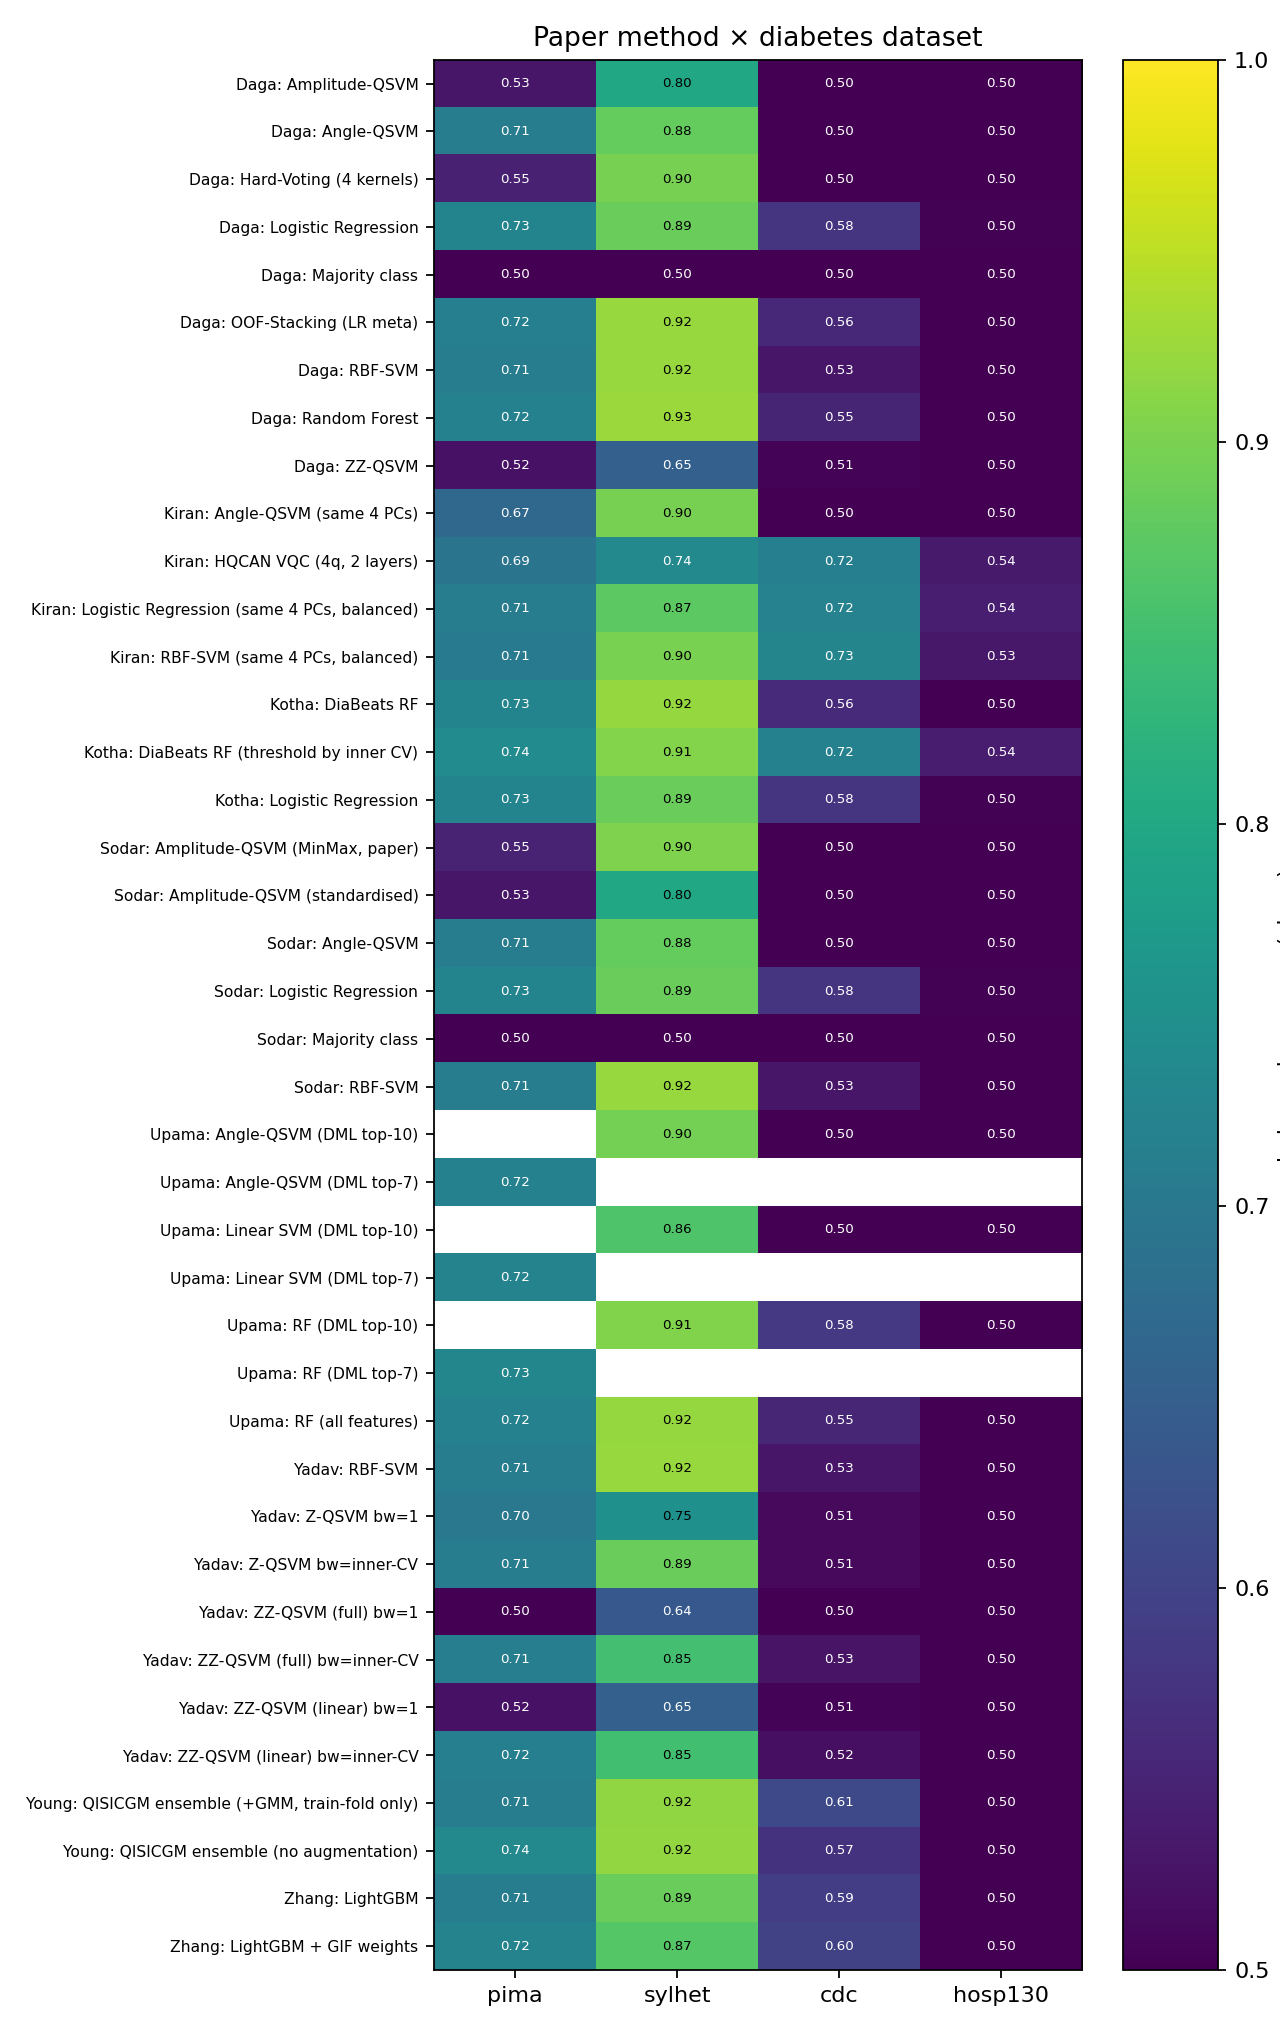
\includegraphics[width=\linewidth,height=0.74\textheight,keepaspectratio]{09_heatmap_balanced_accuracy.png}

    \column{0.41\textwidth}
      \begin{tikzpicture}[font=\scriptsize,c/.style={draw=none,rounded corners=3pt,text width=5.2cm,inner sep=5pt,align=left}]
        \node[c,fill=qgreen!15](a){%
          \tlC{qgreen}\ \textbf{1. Easy Zone (Sylhet):}\\
          Symptoms give $0.85\text{--}0.93$ balanced accuracy across all classical and tuned models.
        };
        \node[c,fill=qamber!15,below=4pt of a](b){%
          \tlC{qamber}\ \textbf{2. Biological Ceiling (Pima):}\\
          Every model plateaus at $0.71\text{--}0.74$. Classical models tie or beat quantum.
        };
        \node[c,fill=qcrimson!12,below=4pt of b](d){%
          \tlC{qcrimson}\ \textbf{3. Zero-Recall Floor (CDC/Hosp):}\\
          Unweighted quantum kernels form a solid block at \textbf{0.500} (chance).
        };
      \end{tikzpicture}
      \vspace{4pt}
      {\tiny Heatmap generated directly from notebook execution results (\texttt{09\_summary.ipynb}).}
  \end{columns}
  \pBfoot{Balanced accuracy scale: yellow/green = high ($>0.80$), purple/blue = chance ($0.50$). Pima, Sylhet, CDC, Hospital 130 = four audited diabetes cohorts. All evaluations clean, leakage-free 15 folds.}
\end{frame}
